\documentclass[b5paper]{article}
% Add "final" option in the article to remove todo
\usepackage[tight,common_math_textnormal,todonotes,math_base_note,math_simple]{gatmeo}
\usepackage{tikz-cd}
\geometry{paperwidth=6.9in, paperheight=9.2in}
\newcommand{\mathintitle}[1]{\texorpdfstring{$#1$}{\detokenize{#1}}}

\title{\bf{
Hypertoric Varieties Arose from Graphs
}}

\newcommand{\noskipline}{\vspace{-1.5em}}

\newcommand{\II}{\mathcal{I}}
\newcommand{\BB}{\mathcal{B}}

\renewcommand{\epsilon}{\varepsilon}
\renewcommand{\phi}{\varphi}
\newcommand{\NN}{\mathbb{N}}
\newcommand{\ZZ}{\mathbb{Z}}
\tikzcdset{
    cells={font=\everymath\expandafter{\the\everymath\displaystyle}},
}

% Hypertoric Variety
\newcommand{\MM}{\mathcal{M}}
\newcommandx*\Mper[1][1=\Gamma]{\mathcal{M}^{\mathrm{per}}(#1)}
\newcommandx*\Mperchar[2][2=\Gamma]{\mathcal{M}^{\mathrm{per}}_{#1}(#2)}
\newcommandx*\Hper[1][1=\Gamma]{\mathcal{A}^{\mathrm{per}}(#1)}
\newcommandx*\Hperchar[2][2=\Gamma]{\mathcal{A}^{\mathrm{per}}_{#1}(#2)}
\newcommandx*\Rper[2][1=\bullet, 2=\Gamma]{\mathcal{R}_{\mathrm{per}}^{#1}(#2)}
\newcommandx*\SRper[2][1=\bullet, 2=\Gamma]{\mathcal{SR}_{\mathrm{per}}^{#1}(#2)}
\newcommandx*\Mfin[1][1=\Gamma]{\mathcal{M}(#1)}
\newcommandx*\Mfinchar[2][2=\Gamma]{\mathcal{M}_{#1}(#2)}
\newcommandx*\Hfinchar[2][2=\Gamma]{\mathcal{A}_{#1}(#2)}
\newcommandx*\Hfin[1][1=\Gamma]{\mathcal{A}(#1)}
\newcommandx*\Rfin[2][1=\bullet, 2=\Gamma]{\mathcal{R}^{#1}(#2)}
\newcommandx*\SR[2][1=\bullet, 2=\Gamma]{\mathcal{SR}^{#1}(#2)}
\newcommandx*\Mmul[1][1=\Gamma]{\mathcal{M}^{\mathrm{mul}}(#1)}
\newcommandx*\idealIper[1][1=\Gamma]{I_{\mathrm{per}}(#1)}
\newcommandx*\idealI[1][1=\Gamma]{I(#1)}
\newcommand{\opendisc}{\mathbb{D}}
\newcommandx*\Betti[1][1=\Gamma]{\mathfrak{B}(#1)}
\newcommandx*\Dolbeault[1][1=\Gamma]{\mathfrak{D}(#1)}

% Core and Toric
\newcommandx*\corefin[1][1=\Gamma]{\mathcal{L}(#1)}
\newcommandx*\coreper[1][1=\Gamma]{\mathcal{L}^{\mathrm{per}}(#1)}
\newcommandx*\toricP[1][1=P]{\mathcal{X}(#1)}
\newcommandx*\fixptP[1][1=B]{P_{#1}}
\newcommandx*\toricB[1][1=B]{\mathcal{X}(#1)}

% Complex
% Group Cohomology Complex
\newcommand{\pGC}{\mathfrak{C}} 
\newcommandx*\GC[3][1=\bullet,2=\bullet,3=\Gamma]{\mathfrak{C}^{#1,#2}(#3)} % Our complex: Group Cohomology
\newcommand{\dGC}{\delta} % Our complex: Group Cohomology
\newcommand{\dGCbar}{\bar{\delta}} % Our complex: Group Cohomology
\newcommand{\fGC}{\phi}
\newcommand{\gGC}{\psi}
\newcommand{\hGC}{\eta}
%--- Group Cohomology Complex with e
\newcommandx*\GCe[4][1=\bullet,2=\bullet,3=\Gamma,4=e]{\mathfrak{C}^{#1,#2}(#3,#4)}
\newcommand{\dGCe}{\delta_e}
\newcommand{\fGCe}{\mathfrak{f}}
\newcommand{\gGCe}{\mathfrak{g}}
\newcommand{\hGCe}{\mathfrak{h}}
%--- CKS
\newcommandx*\GCS[2][1=\bullet,2={\Gamma, S}]{\mathfrak{D}^{#1}(#2)}
\newcommandx*\dGCS[1][1=S]{\dGC_{#1}}
\newcommandx*\fGCS[1][1=S]{\fGC_{#1}}
\newcommandx*\gGCS[1][1=S]{\gGC_{#1}}
\newcommandx*\hGCS[1][1=S]{\hGC_{#1}}
\newcommandx*\CKS[4][1=\bullet,2=\bullet,3=\bullet,4=\Gamma]{\mathfrak{C}^{#1,#2,#3}(#4)} % CKS
\newcommandx*\grCKS[4][1=\bullet,2=\bullet,3=\bullet,4=\Gamma]{I^{#1, #2}\mathfrak{C}^{#3}(#4)} % CKS
\newcommandx*\CKSdiffgrading[3][1=\bullet,2=\bullet,3=\Gamma]{\mathfrak{C}'^{#1,#2}(#3)} % CKS
\newcommand{\dCKS}{d} %CKS Complex
\newcommand{\fCKS}{f}
\newcommand{\gCKS}{g}
\newcommand{\hCKS}{h}
\newcommandx*\HT[3][1=\bullet,2=\bullet,3=\Gamma]{\mathfrak{K}_{\mathrm{per}}^{#1, #2}(#3)}
\newcommandx*\grHT[3][1=\bullet,2=\bullet,3=\Gamma]{I^{#1}\mathfrak{K}_{\mathrm{per}}^{#2}(#3)}
\newcommand{\dHT}{\dCKS_{\mathrm{per}}}
\newcommandx*\HTalt[2][1=\bullet,2=\Gamma]{\tilde{\mathfrak{K}}^{#1}(#2)}
\newcommand{\dHTalt}{\tilde{\dCKS}_{\mathrm{per}}}
\newcommand{\fHT}{\fCKS_{\mathrm{per}}}
\newcommand{\gHT}{\gCKS_{\mathrm{per}}}
\newcommand{\hHT}{\hCKS_{\mathrm{per}}}
\newcommandx*\HTfin[3][1=\bullet,2=\bullet,3=\Gamma]{\mathfrak{K}^{#1, #2}(#3)}
\newcommandx*\grHTfin[3][1=\bullet,2=\bullet,3=\Gamma]{I^{#1}\mathfrak{K}^{#2}(#3)}
\newcommand{\dHTfin}{\dCKS}
\newcommand{\fHTfin}{\fCKS}
\newcommand{\gHTfin}{\gCKS}
\newcommand{\hHTfin}{\hCKS}
\newcommandx*\CPX[3][1=\bullet,2=\bullet,3=\Gamma]{\mathfrak{D}^{#1,#2}(#3)} % Intermediate complex
\newcommandx*\euler[3][3=\Gamma]{\eta^{#1, #2}(#3)}

% Graph and Matroids
\newcommandx*\Tutte[2][1=\Gamma]{T(#1;\, #2)}
\newcommandx*\hpoly[2][1=\Gamma]{h(#1;\, #2)}
\newcommandx*\HTutte[2][1=\Gamma]{H(#1;\, #2)}
\newcommandx*\seqn[1][1=n]{[-#1,#1]}
\newcommand{\loopgraph}{{\bigcirc\!\!\bullet}}
\newcommand{\bridgegraph}{{\bullet\mspace{-7mu}-\mspace{-7mu}\bullet}}
\newcommand{\supnorm}[1]{\| #1 \|_{\infty}} 

\newcommand{\del}{\setminus}
\newcommand{\con}{\mathbin{/}}
\newcommand{\Gammaper}{\Gamma_{\mathrm{per}}}
\newcommandx*\tree[2][2=\Gamma]{\mathcal{T}_{#2}(#1)}
\newcommandx*\treefunction[1][1=\Gamma]{\mathcal{T}_{#1}}
\newcommandx*\cotreefunction[1][1=\Gamma]{\mathcal{T}_{#1}^*}
\newcommandx*\cotree[2][2=\Gamma]{\mathcal{T}_{#2}^*(#1)}
\newcommandx*\face[2][1=\bullet,2=\Gamma]{F_{#1}(#2)}
\newcommandx*\faceshelling[3][2=\bullet,3=\Gamma]{F_{#2}^{(#1)}(#3)}
\newcommandx*\faceper[2][1=\bullet,2=\Gamma]{F^{\mathrm{per}}_{#1}(#2)}
\newcommandx*\pair[3][3=\Gamma]{\langle #1, #2 \rangle_{#3}}
\newcommandx*\cotreein[2][2=\Gamma]{\mathcal{D}_{#2}(#1)}
\newcommandx*\cotreeinper[2][2=\Gamma]{\mathcal{D}^\per_{#2}(#1)}
\newcommandx*\cotreeinfunction[1][1=\Gamma]{\mathcal{D}_{#1}}
\newcommandx*\externalactivity[2][2=\Gamma]{EA_{#2}(#1)}
\newcommandx*\internalactivity[2][2=\Gamma]{IA_{#2}(#1)}
\newcommand{\intp}[1]{\iota_{#1}} % interior product
\newcommandx*\fundcycle[2][2=\Gamma]{\gamma_{#1}}
\newcommandx*\fundcyclewithtree[2][2=B]{\gamma_{#2,#1}}
\newcommandx*\fundbond[2][2=\Gamma]{\beta_{#1}}
\newcommandx*\fundbondwithtree[2][2=B]{\beta_{#2^*,#1}}
\newcommandx*\basis[2][1=\bullet,2=\Gamma]{\mathcal{B}_{#1}(#2)}
\newcommandx*\basisper[2][1=\bullet,2=\Gamma]{\mathcal{B}^\per_{#1}(#2)}

\newcommandx*\SE[3][1=,3=]{
  \ifstrempty{#3}
  {\ifstrempty{#1}{E^\bullet_{#2}}{#1_{#2}}}
  {\ifstrempty{#1}{E_{#2}(#3)}{#1_{#2}}}
}
\newcommandx*\HMGZ[2][1=\Gamma,2=\bullet]{H^{#2}(\MM(#1),\mathbb{Z})}
\newcommand{\hCCC}{\hat{\mathfrak{C}}}

\newcommand{\per}{\mathrm{per}}

% Math Operations
\newcommand{\HH}{\mathrm{H}}
\newcommandx*\Ext[1][1=\bullet]{\bigwedge\nolimits^{#1}}
\newcommandx*\Sym[1][1=\bullet]{\mathrm{Sym}^{#1}}
\newcommand{\sgn}{\mathrm{sgn}}
\newcommand{\coker}{\operatorname{coker}}
\renewcommand{\im}{\operatorname{Im}}
\newcommand{\supp}{\mathrm{supp}}
\newcommand{\Hom}{\mathrm{Hom}}

% Group Cohomology
\newcommand{\invar}[1]{\Gamma_{#1}}
\newcommandx*\Rder[1][1=\bullet]{R^{#1}}
\newcommandx*\totRder[1][1=\bullet]{\mathbb{R}^{#1}}

% Homotopy Equivalence
\newcommand{\choice}[1]{[#1]} % choice for HTfin equiv
\newcommandx*\intord[2][2=S]{[#2]^{#1}} % integration order for GCS equiv
\newcommandx*\hyppl[2][2=S]{\alpha^{#2}_{#1}} % hyperplane for GCS equiv

\makeatletter
\newcommand{\GIT}[1][\@nil]{%
  \def\tmp{#1}%
  \ifx\tmp\@nnil
    /\!\!/%
  \else
    /\!\!/_{\! #1}%
  \fi
}
\newcommand{\HQ}[1][\@nil]{%
  \def\tmp{#1}%
  \ifx\tmp\@nnil
    /\!\!/\!\!/\!\!/%
  \else
    /\!\!/\!\!/\!\!/_{\! #1}%
  \fi
}
\makeatother

\newcommand{\Diff}{\mathrm{Diff}}
\newcommand{\Sympl}{\mathrm{Sympl}}
\newcommand{\acton}{\curvearrowright}
\newcommand{\smth}{C^\infty}
\newcommand{\df}{\Omega}
\newcommand{\vf}{\mathrm{Vec}}
\newcommand{\svf}{\mathrm{Vec}_\mathrm{sym}}
\newcommand{\hvf}{\mathrm{Vec}_\mathrm{ham}}
\newcommand{\ind}[1]{#1^\#}
\newcommand{\lied}[1]{\mathcal{L}_{#1}}
\newcommand{\intd}[1]{\iota_{#1}}
\newcommand{\Proj}{\textnormal{Proj }}
\newcommand{\Spec}{\textnormal{Spec }}
\newcommand{\sstab}{\mathrm{ss}}
\newcommand{\pstab}{\mathrm{ps}}
\newcommand{\stab}{\mathrm{s}}
\newcommand{\Stab}{\textnormal{Stab}}
\newcommand{\cork}{\textnormal{cork}}
\newcommand{\Chbar}{\mathbb{C}^\times _\hbar}

\begin{document}
\maketitle
\vspace{-3.5em}
%\input{abstract}

\thispagestyle{empty}
\tableofcontents
\listoftodos

\section{Symplectic Reduction for Toric Varieties}

\subsection{Symplectic Reduction for Hamiltonian Action}

Consider a Lie group $G$ acting on a manifold $M$. For $X\in\mathfrak{g}$, denote $\ind{X}$ the induced vector field on $M$. If we assume $M$ is symplectic and $G$ acts symplectically, i.e. $G$ preserve symplectic form, the action is Hamiltonian if there also exists a moment map $\mu : M \to \mathfrak{g}^*$ such that
\begin{enumerate}
    \item $\mu$ is $G$-equivariant where $G$ acts on $\mathfrak{g}^*$ by the coadjoint action, and
    \item for all $X \in \mathfrak{g}$, considered as $X : \mathfrak{g}^* \to \mathbb{R}$, $d(X \circ \mu) = \omega(\cdot ,\ind{X})=-\intd{\ind{X}}\omega$.
\end{enumerate}
Notice that we use the convention that flipped the sign for the interior product.

If $G$ is abelian, then any shift $\mu+\alpha$, $\alpha\in\mathfrak{g}^*$, is also a moment map.

\begin{example}[exp:Cn_moment]{$\mathbb{T}_\mathbb{R}^n \acton \mathbb{C}^n$}
    Consider the real torus $\mathbb{T}_\mathbb{R}^n=(S^1)^n$ acting on $\mathbb{C}^n$ by rotating each coordinate. There is a canonical real symplectic form on $\mathbb{C}^n$ given by $\omega_\mathbb{R}=\sum_jdx_j\wedge dy_j$. Let $X_i\in\mathfrak{t}_\mathbb{R}^n$ be a standard basis vector, 
    the induced vector field $\ind{X_i}$ is given by
    \begin{align*}
        (\ind{X_i})_z &= \frac{d}{dt} [e^{it} z_i]_{t=0}
        = \frac{d}{dt} [(\cos(t) x_i - \sin(t) y_i,\sin(t)x_i + \cos(t)y_i)]_{t=0}
        = -2y_i \left.\frac{\partial}{\partial x_i}\right|_z + 2x_i \left.\frac{\partial}{\partial y_i}\right|_z.\\
        \intd{\ind{X_i}}\omega_\mathbb{R} &= \biggl(\sum_j dx_j \wedge dy_j\biggr)\left(-2 y_i \frac{\partial}{\partial x_i} + 2 x_i \frac{\partial}{\partial y_i}\right)
        = -2 (x_i \, dx_i + y_i \, dy_i).
    \end{align*}
    Thus, $-\intd{\ind{X_i}}\omega_\mathbb{R} = d(x_i^2 + y_i^2) = d(|z_i|^2)$. Note that $X_i : (\mathfrak{t}^n)^* \to \mathbb{R}$ is regarded as the $i$th coordinate map. It follows that $\mu(z_1, \dots, z_n) = (\pi|z_1|^2, \dots, \pi|z_n|^2)$ is a choice of moment map.
\end{example}

It is easy to check that $\mu^{-1}(\xi) \subseteq M$ for any $\xi$ in the center of $\mathfrak{g^*}$ is $G$-invariant. Choose $\xi=0$, we define $M\GIT G=\mu^{-1}(0)\GIT G$ to be the symplectic reduction of $M$ by $G$ if $G$ acts on $\mu^{-1}(0)$ is free. In particular, if $G$ is abelian, we can do the reduction at different moment map level $\mu^{-1}(\xi)$.

\begin{theorem}{Marsden-Weinstein-Meyer Theorem}
    Assume that the restricted action $G $ on $ \mu^{-1}(0)$ is free. Let $\iota:\mu^{-1}(0)\rightarrow M$. Then,
    \begin{enumerate}
        \item $M \GIT G$ is a smooth manifold and $\pi:\mu^{-1}(0) \to M \GIT G$ is a principal bundle, and
        \item there is a symplectic form $\omega_{\mathrm{red}}$ on $M \GIT G$ satisfying $\iota^*\omega = \pi^*\omega_{\mathrm{red}}$.
    \end{enumerate}
\end{theorem}

\subsection{Symplectic Toric Manifold}

We define a symplectic toric manifold to be a compact connected $2n$-dimensional symplectic manifold $M$ with an effective real $n$-dimensional torus Hamiltonian action $T$, i.e. $T \to \Sympl(M)$ is injective.
We will see later that such spaces can be described using Delzant Polytopes, which correspond to complex $n$-dimensional connected projective toric varieties.

Let $\Delta \subseteq (\mathbb{R}^d)^*$ be a rational convex polytope with $n$ facets.
Such a polytope is said to be
\begin{itemize}
    \item \vocab{simple} if there are $d$ edges meeting at each vertex,
    \item \vocab{unimodular} if for all vertex $x$, there exist $v_1, \dots, v_n \in \mathbb{Z}^d$ that spans the $d$ edges such that $(v_1, \dots, v_d)$ forms a $\mathbb{Z}$-basis of $\mathbb{Z}^d$, and
    \item \vocab{Delzant} if it is rational, simple, and unimodular.
\end{itemize}
If we describe $\Delta$ as the intersection of $n$ affine hyperplanes, i.e. there exists normal vectors $a_i\in \mathbb{Z}^d$ and shifts $r_i\in\mathbb{R}$ such that 
\begin{equation*}
    \Delta = \{ x \in (\mathbb{R}^d)^* \mid \langle x, a_i \rangle + \theta_i \leq 0 \  \forall\ 1 \leq i \leq n \},
\end{equation*}
we can translate the above terminology: a hyperplane arrangement is said to be
\begin{itemize}
    \item \vocab{simple} if every $k$ hyperplanes with non-empty intersection intersect at codimension $k$;
    \item \vocab{unimodular} if every collection of $d$ independent vectors in $\{a_i\}$ forms a $\mathbb{Z}$-basis of $\mathbb{Z}^d$.
\end{itemize}
Let $\pi:\mathbb{Z}^n\rightarrow \mathbb{Z}^d$ be the $\mathbb{Z}$-linear map which sends the $i$-th basis vector to $a_i$. Unimodularity implies $\pi$ is surjective. Let $\mathbb{Z}^k$ be the kernel of $\pi$ where $k=n-d$, we have the following exact sequence:
\begin{equation}
  \label{eq:exact_seq_Z}
  \begin{tikzcd}[row sep=small]
    1 \arrow[r] & \mathbb{Z}^k \arrow[r, "\iota"] & \mathbb{Z}^n \arrow[r, "\pi"] & \mathbb{Z}^d \arrow[r] & 1.
  \end{tikzcd}
\end{equation}

Unimodularity also implies that the maximal minors of the matrix $\left[a_1|\dots|a_n\right]$ for $\pi$ are $0,\pm1$. In fact, one can check that the RREF of $\left[a_1|\dots|a_n\right]$ is totally unimodular, i.e. all minors are $0,\pm1$.

\begin{theorem}{}
  There is a one-to-one correspondence between Delzant polytopes and symplectic toric manifolds $(M, \omega, \mathbb{T}^d, \mu)$. In particular, $\im(\mu) \subseteq (\mathbb{R}^d)^*$ is a Delzant polytope. 
  \begin{proof}
    With the notation above, we claim that with a Delzant polytope $\Delta$, we can associate a symplectic toric manifold $M=\mathbb{C}^n \GIT \mathbb{T}^k$.
    \Cref{eq:exact_seq_Z} induces the following exact sequence of tori and lie algebras:
    \begin{equation*}
      \begin{tikzcd}[row sep=small]
        1 \arrow[r] & \mathbb{T}^k \arrow[r, "\iota"] & \mathbb{T}^n \arrow[r, "\pi"] & \mathbb{T}^d \arrow[r] & 1 \\
        0  & (\mathfrak{t}^k)^* \arrow[l] & (\mathfrak{t}^n)^* \arrow[l, "\iota^*"] & (\mathfrak{t}^d)^* \arrow[l, "\pi^*"] & 0\arrow[l].
      \end{tikzcd}
    \end{equation*}
    Consider the standard action $\mathbb{T}^n $ on $\mathbb{C}^n$ with moment map (\Cref{exp:Cn_moment}) $\mu : \mathbb{C}^n \to (\mathfrak{t}^n)^*$,
    \begin{equation*}
      \mu(z_1, \dots, z_n) = (|z_1|^2 - \theta_1, \dots, |z_n|^2 - \theta_n).
    \end{equation*}
    The inclusion $\iota$ induces an action $\mathbb{T}^k$ on $\mathbb{C}^n$, with moment map given by the composite $\iota^* \circ \mu : \mathbb{C}^n \to (\mathfrak{t}^k)^*$. This allows us to define the symplectic reduction $M = \mathbb{C}^n \GIT \mathbb{T}^k$. 
    \begin{itemize}
      \item $Z:=(\iota^*\circ \mu)^{-1}(0)=\mu^{-1}(\pi^*(\Delta))$ is compact: Consider $\pi^*:(\mathfrak{t}^d)^*\rightarrow (\mathfrak{t}^n)^*$ as the transpose of $\pi$. $\im(\pi^*)=\ker(\iota^*)\subseteq (\mathfrak{t}^n)^*$ is a $d$-dimension linear subspace cut out by the equation of $\iota^*$. Recall $\Delta$ is the intersection of half space $\CB{x\in (\mathfrak{t}^d)^*\mid \AB{x,\pi(e_i)}+\theta_i\leq 0}$. $\pi^*(\Delta)\subseteq \im(\pi^*)$ then equals the intersection of half space $\CB{x\in \im(\pi^*)\subseteq (\mathfrak{t}^n)^*\mid \AB{x,e_i}+\theta_i\leq 0}$. Hence 
        \[
          (\iota^*\circ \mu)^{-1}(0)=\mu^{-1}(\ker(\iota^*))=\mu^{-1}(\im(\pi^*))=\mu^{-1}(\pi^*(\Delta))
        \]
        is compact as $\mu$ is proper.
      \item $T^k$ acts freely on $Z$: For $z\in Z$, let $I_z=\CB{i\mid z_i=0}$. The stablelizer 
        \[
          T^n_z=\CB{t\in T^n\mid t_i=1\textnormal{ if }i\notin I_z}\simeq T^{I_z}.
        \]
        Recall $\mu_i(z)=|z_i|^2-\theta_i$, $z_i=0$ iff $\AB{\mu(z),e_i}+\theta_i=0$ iff $\AB{x,\pi(e_i)}+\theta_i=0$ for some $x\in \Delta$. Hence $I_z$ is the set of hyperplanes where $\mu(z)$ lies on. In particular, $|I_z|\leq d$. Since $\CB{\pi(e_i)\mid i\in I_z}$ is linearly independent, $\pi:T^n_z\rightarrow T^d$ is injective. Hence $T^k$ acts freely on $Z$.
    \item Moment polytope of $M$ is $\Delta$: The $T^d$ fix points of $M$ by the above discussion is hence the vertices of $\Delta$. We omit the remaining of the proof.
    \end{itemize}
  \end{proof}
\end{theorem}

In fact, the polytope $\pi^*(\Delta)=\ker(\iota^*)\bigcap_i \CB{x_i+\theta_i\leq 0}$ can be shifted to the intersection of $\bigcap_i \CB{x_i\leq 0}$ with a affine subspace $\im(\pi^*+\theta)=\ker(\iota^*-\iota^*(\theta))$. Hence in order to describe $\pi^*(\Delta)$, it is suffice to specify an element $\iota^*(\theta)\in (\mathfrak{t}^k)^*$. The moment map also depends only on $\iota^*(\theta)$ instead of $\theta$. In other words, to define a symplectic toric variety, we can choose the standard moment map $\mu_\textnormal{std}(z)=(|z_1|^2, \dots, |z_d|^2)$, and the reduction is can be defined by $\lambda=\iota^*(\theta)\in \mathfrak{t}^*$ as
\[
  M = \mathbb{C}^n \GIT \mathbb{T}^k = \mu_\textnormal{std}^{-1}(\lambda).
\]

\begin{example}{}
    Consider the following polytope.
    \begin{equation*}
        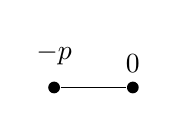
\begin{tikzpicture}[every node/.style={circle,fill=black,minimum width=1.5pt,inner sep=1.5pt}]
            \node[label={$-p$}] (A) at (0,0) {};
            \node[label={$0$}] (B) at (1,0) {};
            \draw (A) -- (B);
        \end{tikzpicture}
        \implies
        \begin{aligned}
            a_0 &= -1 & \theta_0 &= p \\
            a_1 &= 1 & \theta_1 &= 0
        \end{aligned}
    \end{equation*}
    $\mathbb{T}^1$ acts on $\mathbb{C}^2$ by $\lambda \cdot (z_1, z_2) = (\lambda z_1, \lambda z_2)$. $\pi=(-1,1)$ and $\iota=(1,1)^T$.
    The moment map $\iota^* \circ \mu : \mathbb{C}^2 \to (\mathfrak{t}^1)^*$ is given by
    \begin{equation*}
        \iota^*(\mu(z_1, z_2)) = \iota^*(|z_1|^2-p, |z_2|^2) = (|z_1|^2+|z_2|^2) - p.
    \end{equation*}
    Thus, $Z = (\iota^* \circ \mu)^{-1}(0) = (\iota^* \circ \mu_\textnormal{std})^{-1}(p) = \{ z \in \mathbb{C}^2 \mid |z|^2 = p\}$. Hence $Z\simeq \mathbb{C}^2 / \mathbb{R}_{>0}$, $Z/\mathbb{T}^1 \cong \mathbb{P}^1$.

    For $\mathbb{P}^n$, consider the polytope
    \begin{equation*}
        \mathrm{conv}(\{ 0, e_1, \dots, e_n \})
        \implies
        \begin{aligned}
            a_0 &= (-1, \dots, -1) & \theta_0 &= p \in \mathbb{Z}_{>0} \\
            a_i &= e_i & \theta_i &= 0 \quad \forall 1 \leq i \leq n
        \end{aligned}
    \end{equation*}
    $\iota=(1,\dots ,1)^T$.
    Similarly, $\iota^* \circ \mu : \mathbb{C}^3 \to (\mathfrak{t}^1)^*$ is given by
    $\iota^*(\mu(z_0, \dots, z_n)) = (|z_0|^2+\cdots+|z_n|^2) - p$.
    $Z = (\iota^* \circ \mu)^{-1}(0) = \{ z \in \mathbb{C}^{n+1} \mid |z|^2 = p\}=\mathbb{C}^{n+1} / \mathbb{R}_{>0}/\mathbb{T}^1 \cong \mathbb{P}^n$.
\end{example}

\subsection{Toric as GIT Quotient}

\label{sec:symplectic_reduction_as_git}

Write $G=(\mathbb{C}^\times )^k$, let character $\chi:G\rightarrow \mathbb{C}^\times $.
Let $L_{\chi^r}$ to be the linearized line bundle with character $\chi$, i.e. the sheaf of sections of $\mathbb{C}^n\times \mathbb{C}$ with $G$ action $g(p,t)=(g\cdot p,\chi(g)t)$.
Define the GIT quotient
\[
  \mathbb{C}^n\GIT_\chi:=\textnormal{Proj}\bigoplus _{r=0}^{\infty }\HH^0(\mathbb{C}^n,L_{\chi^r})^G=\textnormal{Proj}\bigoplus _{r=0}^{\infty }\CB{f\in \mathbb{C}[x_i]\mid f(g\cdot p)=\chi(g)^rf(p)\ \forall\ g\in G}.
\]
The Proj construction is defined on graded ring $S=\bigoplus _{n=0}^{\infty }S_n$ where $S_nS_m=S_{n+m}$. Let $S_+=\bigoplus _{n>0}S_n$. We denote $\textnormal{Proj}S\subseteq \textnormal{Spec}S$ to be the set of homogeous prime ideal $\mathfrak{p}$ s.t. $S_+\not\subseteq \mathfrak{p}$. Here, $\chi$ gives the grading on $\mathbb{C}[x_i]$ to talk about homogenousity.

\begin{example}[exp:GIT_P1_Proj]{}
  Consider the diagonal action $\mathbb{C}^*$ acting on $\mathbb{C}^2$. Let $\chi:G\rightarrow \mathbb{C}^\times$ be the identity, giving the standing grading on $S=\mathbb{C}[\mathbb{C}^2]=\mathbb{C}[x,y]$. Points in $\textnormal{Spec}S$: 
  \begin{itemize}
    \item $(0)$ is in $\Proj S$.
    \item Closed points are $(x-a,y-b)$. Homogenous implies $a=b=0$, yet $(x,y)=S_+$ is not in $\Proj S$.
    \item Irreducible homogenous prime ideals are $(ax+by)$, giving a $\mathbb{P}^1$ family of points in $\Proj S$.
  \end{itemize}
  The closed points in $\Proj S$ should then be thought of as maximal ideal in $\Proj S$, which corresponding to lines $k(ax+by)$ in $\Spec S$.

  Note that changing $\chi$ will be changing the grading, and hence $\Proj S$. A degenerate case is $\chi:(g)\mapsto 1$. The only invariant functions are constant functions. Hence $\Proj S=\Spec \mathbb{C}$ is a point.
\end{example}

A geometric way to understand GIT is by stability.
\begin{definition}[def:]{}
  Fix $G\subseteq (\mathbb{C}^\times )^n$ and character $\chi$ with linearized line bundle $L_\chi$. $p\in \mathbb{C}^n$ is
  \begin{itemize}
    \item semistable if there are $r>0$, $f\in \HH^0(\mathbb{C}^n,L_\chi^r)^G$ s.t. $f(p)\neq 0$,
    \item polystable if semistable with $G$-orbits closed in the semistable locus,
    \item stable if semistable and $G_p$ is finite with $G$-orbits closed in $\mathbb{C}^n_f=\CB{p\in \mathbb{C}^n\mid f(p)\neq 0}$.
    \item unstable if not semistable.
  \end{itemize}
  Denote $(\mathbb{C}^n)^{\chi-\sstab}$ and $(\mathbb{C}^n)^{\chi-\stab}$ to be the set of semistable points and stable points respectively.
\end{definition}
The reason why it is geometric is because of the following theorem:
\begin{theorem}[thm:]{}
  Let $G\subseteq (\mathbb{C}^\times )^n$.
  $\mathbb{C}^n\GIT_\chi G=(\mathbb{C}^n)^{\chi-\sstab}\GIT G:=\Spec(\mathbb{C}[(\mathbb{C}^n)^{\chi-\sstab}]^G)$.
\end{theorem}

\begin{example}[exp:]{}
  Back to \Cref{exp:GIT_P1_Proj},  for $\chi:G\rightarrow \mathbb{C}^\times $ be the identity, every points $p$ except $(0,0)$ exists a homogeous function $f:(x,y)\mapsto x+y$ and $r=1$ that does not vanish at $p$. One need to then check that a good categorical quotient of $\mathbb{C}^2\setminus \{0\}$ is $\mathbb{P}^1$. For trivial $\chi$ on the other hand, constant function serve as the required homogenous function for every point. $G$ orbits of in $\mathbb{C}^2$ are lines removing the origin. All their closure intersect at origin. The categorical quotient on $\mathbb{C}^2$ is hence $\Spec \mathbb{C}[x_1,x_2]^G=\CB{\textnormal{pt}}$.
\end{example}

\subsection{Relating Symplectic Reduction and GIT}

\missing{Frances Kirwan's thesis}
%http://www.cms.zju.edu.cn/UploadFiles/AttachFiles/201096185821505.pdf

\section{Hypertoric Varieties}
\subsection{As symplectic Reduction}

Hypertoric varieties is defined similar to the symplectic reduction construction for toric varieties $\mathbb{C}^n\GIT T_\mathbb{R}^k$. However, the fundamental building block changed to complex torus $T=\mathbb{C}^*$ acting on $T^*\mathbb{C}$ instead of $T_\mathbb{R}$ acting on $\mathbb{C}$; we consider general hyperplane arrangement instead of those arise from polytope; and the $(\mathbb{C}^*)^k$ action on $\mu^{-1}(0)$ may no longer be free. First, the moment map.
\begin{example}[exp:]{$(\mathbb{C^*})^n\acton T^*\mathbb{C}^n$}
  The $D=(\mathbb{C}^*)^n$-action on $T^*\mathbb{C}^n$ is given by $(t_iz_i,t^{-1}w_i)_{i=1}^{n}$.
  There is a canonical complex symplec form on $T^*\mathbb{C}^n$ by $\omega=\sum_{i}^{}dw_i\wedge dz_i$. Let $X_i\in \mathfrak{d}^n$ be a standard basis,
  \begin{alignat*}{1}
    (\ind{X_i})_z&=\frac{d}{dt}[e^{t_i}z_i,e^{-t_i}w_i]_{t=0}=z_i\frac{\partial }{\partial z_i}-w_i\frac{\partial }{\partial w_i},\\
    \iota_{\ind{X_i}}\omega&= \left(\sum_{}^{}dw_i\wedge dz_i\right)\left(z_i\frac{\partial }{\partial z_i} - w_i\frac{\partial }{\partial w_i}\right)=-\sum z_idw_i + w_idz_i.
  \end{alignat*}
  Thus, $-\intd{\ind{X_i}}\omega = z_idw_i+w_idz_i = d(z_iw_i)$, $\mu(z_1,w_1,\dots ,z_n,w_n)=\sum_{}^{}z_iw_i$ is a moment map.
\end{example}

Given a short exact sequence of complex tori
\begin{equation}
  \label{eq:exact_seq_tori}
    \begin{tikzcd}
        1 \arrow[r] & G \arrow[r, "\iota"] & D \arrow[r, "\pi"] & T \arrow[r] & 1
    \end{tikzcd}
\end{equation}
with $ D \cong (\mathbb{C}^\times)^n $, we consider
\begin{enumerate}
    \item the $G$-action on $T^*\mathbb{C}^n$ by $ g \cdot (z, w) = (\iota(g)_iz_i, \iota(g)_i^{-1}w_i)_{i=1}^n $, and
    \item the moment map $ \mu : T^*\mathbb{C}^n \to \mathfrak{g}^* $ for the $G$-action given by $ (z, w) \mapsto \iota^*((z_iw_i)_{i=1}^n) $.
\end{enumerate}
Similar to above, $\iota:G\rightarrow D$ and a choice of $ \lambda \in \mathfrak{g}^* $ define the symplectic reduction of $T^*\mathbb{C}^n$ by $G$ as the quotient $\mu^{-1}(\lambda)$ by $G$. However, $G$ may not act freely on $\mu^{-1}(\lambda)$, and hence we need further pick a character $ \chi : G \to \mathbb{C}^\times $ and define the hypertoric variety to be the GIT quotient
\begin{equation*}
  \mathcal{M}_{\chi, \lambda} = T^*\mathbb{C}^n \HQ[\chi, \lambda] G = \mu^{-1}(\lambda) \GIT[\chi] G:=\textnormal{Proj}\bigoplus _{r=0}^{\infty }\CB{f\in \textnormal{Fun}(\mu^{-1}(\lambda))\mid f(g\cdot x)=\chi(g)^rf(x)\ \forall\ g}.
\end{equation*}
\begin{example}{$\mathbb{C}^\times \acton T^*\mathbb{C}^{n+1}$}
  Let $G=\mathbb{C}^\times$ and $D=(\mathbb{C}^\times )^{n+1}$ with $\iota:G\rightarrow D$ given by the diagonal map.
    The action $\mathbb{C}^\times$ on $T^*\mathbb{C}^{n+1}$ is given by $\lambda \cdot (z, w) = (\lambda z, \lambda^{-1} w)$. We have
    \begin{align*}
        \mu^{-1}(0) &= \{ (z, w) \in T^*\mathbb{C}^{n+1} \mid z_0w_0 + z_1w_1 + \cdots + z_nw_n = 0 \}.
    \end{align*}
    Let $\chi : \lambda \mapsto \lambda^p$ be the character of $G$.
    We now establish the stability of the action. Note that for all $r>0$, the only function $f$ on $T^*\mathbb{C}^{n+1}$ satisfying $f(0, \lambda^{-1}w)=\lambda^{rp} \, f(0, w)$ for all $\lambda \in \mathbb{C}^\times$ is $f=0$. Thus, $(0, w) \notin (T^*\mathbb{C}^{n+1})^\sstab$. Conversely, suppose $z \neq 0$. Then, we may pick $f(z, w) = z^p$, which satisfies the equation $f(\lambda z, \lambda^{-1}w) = \lambda^p \, f(z, w)$ for all $\lambda \in \mathbb{C}^\times$. Thus, $(z, w)$ is semistable. Moreover, the orbit $T \cdot (z, w)$ is closed in the non-vanishing locus of $f$, and the orbit is clearly of dimension 1. Thus, $(z, w)$ is stable. In conclusion, we have
    \begin{enumerate}
        \item $(T^*\mathbb{C}^{n+1})^\sstab = (T^*\mathbb{C}^{n+1})^\stab = T^*\mathbb{C}^{n+1} \setminus \{ z=0 \}$, and
        \item $\mu^{-1}(0)^\sstab = \mu^{-1}(0)^\stab = \{ (z, w) \mid z_0w_0 + z_1w_1 + \cdots + z_nw_n = 0, z \neq 0 \}$.
    \end{enumerate}

    After taking quotients, we have the following diagram.
    \begin{equation*}
        \begin{tikzcd}
            \mu^{-1}(0)^\stab \arrow[d, hookrightarrow] \arrow[r] & \mu^{-1}(0) \GIT[\chi] \mathbb{C}^\times \arrow[dd, dashed, "\pi"] \\
            (T^*\mathbb{C}^{n+1})^\stab \arrow[d] & {} \\
            \mathbb{C}^{n+1} \setminus \{ 0 \} \arrow[r] & \mathbb{C}^{n+1} \GIT[\chi] \mathbb{C}^\times = \mathbb{P}^n
        \end{tikzcd}
    \end{equation*}
    Note that the composite on the LHS is $\mathbb{C}^\times$-equivariant, thus it descents to the dashed arrow $\pi$. We claim that $T^*\mathbb{C}^{n+1} \HQ[\chi] \mathbb{C}^\times = T^*\mathbb{P}^n$. Note that
    \begin{align*}
        T^*\mathbb{C}^{n+1} \HQ[\chi] \mathbb{C}^\times = \mu^{-1}(0)^\stab / \mathbb{C}^\times = (T^*\mathbb{C}^{n+1} \setminus \{ 0 \}) \GIT \mathbb{C}^\times && \text{since} && \mu^{-1}(0)^\stab = \left(\mu|_{T^*(\mathbb{C}^{n+1} \setminus \{ 0 \})}\right)^{-1}(0).
    \end{align*}
    The claim then follows from Proposition~\ref{prop:cot red} by setting $M = \mathbb{C}^{n+1} \setminus \{ 0 \}$ and $G = \mathbb{C}^\times$.
\end{example}

\begin{proposition}[prop:cot red]{}
  Let $M$ be a smooth manifold with a free and proper $G$-action. This induces a Hamiltonian $G$-action on $T^*M$ with moment map $\mu : T^*M \to \mathfrak{g}^*$. Then, $(T^*M) \GIT G \cong T^*(M/G)$.
  \begin{proof}
    As $G \acton M$ is free and proper, $M/G$ is a smooth manifold. Let $\pi : T^*M \to M$ be the projection and consider the induced action $G$ on $T^*M$. 
    Define the tautological form $\theta \in \df^1(T^*M)$ by
        \begin{equation*}
            \theta_{(p, \alpha)} = d\pi_{(p, \alpha)}^*(\alpha) \quad \text{ i.e.} \quad \theta_{(p, \alpha)}(v) = \alpha(d\pi_{(p, \alpha)}(v))
        \end{equation*}
        for all $p \in M$, $\alpha \in T_p^*M$, $v \in T_{(p, \alpha)}(T^*M)$. Define $\omega = -d\theta$. Then, $(T^*M, \omega)$ is a symplectic manifold. Let $(p_1, \dots, p_n, \alpha^1, \dots, \alpha^n)$ be a local coordinate of $U \subseteq T^*M$. Then, $\theta|_U = \sum_i \alpha^i \, dp_i$ and $\omega|_U = \sum_i d\alpha^i \wedge dp_i$. We claim that the action $G$ on $T^*M$ given by $g\cdot (p,\alpha)=(g\cdot p,d(g^{-1})^*_p(\alpha))$ is hamiltonian with a canonical choice of moment map given by $\mu(p,\alpha)(X)=\alpha(\ind{X_p})$ for all $X \in \mathfrak{g}$.

    Note that we have the following isomorphisms, where $\perp$ denotes the annihilator.
    \begin{align*}
      T_{[p]}(M/G) \cong T_pM / T_p(G \cdot p) && T_{[p]}^*(M/G) \cong T_p(G \cdot p)^\perp \subseteq T_p^*M
    \end{align*}
    Let $\pi : TM \to T(M/G)$ be the projection. Note that $\ker(\pi_p) \cong T_p(G \cdot p)$. Using the fact that $G$ act on $M$ is free, we can show that $\ker(\pi_p) = \{ v \in T_pM \mid \pi(p, v) = 0 \} = \{ \ind{X}_p \mid X \in \mathfrak{g} \} \cong \mathfrak{g}$ for all $p \in M$.

    Let $\tau : (T^*M) \GIT G \to M/G$ be the map induced by the $G$-equivariant map $\mu^{-1}(0) \to M$. Then, $\tau$ is surjective since for all $p \in M$, $(p, 0) \in \mu^{-1}(0)$. Let $p \in M$. Since $G$ acts on $M$ freely, the fiber $\tau^{-1}([p])$ has the following description.
    \begin{align*}
      \tau^{-1}([p]) &= \{ [p, \alpha] \mid (p, \alpha) \in \mu^{-1}(0) \} \\
                     &\cong \{ \alpha \in T_p^*M \mid \mu(p, \alpha) = 0 \} = \{ \alpha \in T_p^*M \mid \alpha(\ind{X}_p) = 0 \quad \forall X \in \mathfrak{g} \} \\
                     &= \{ \ind{X}_p \mid X \in \mathfrak{g} \}^\perp = \ker(\pi_p)^\perp \cong T_p(G \cdot p)^\perp = T_p^*M
    \end{align*}
    This gives the required isomorphism $(T^*M) \GIT G \cong T^*(M/G)$.
  \end{proof}
\end{proposition}

\begin{example}[exp:]{}
  We can also alternatively use the Proj construction. Using a different convention of action $\mathbb{C}^\times $ on $T^*\mathbb{C}^2$ by $\lambda\cdot (z_0,w_0,z_1,w_1)=(\lambda^{-1}z_0,\lambda w_0,\lambda z_1,\lambda^{-1}w_1)$. $S=\mathbb{C}[z_0w_0=z_1w_1]=\mathbb{C}[z_0,w_0,z_1,w_1]/\AB{z_0w_0=z_1w_1}$, where $S_0=\AB{z_0w_0=z_1w_1, z_0z_1,w_0w_1}$, where $(z_0z_1)(w_0w_1)=(z_0w_0)^2$. $\Proj S$ is covered by $w_0\neq 0$ and $z_1\neq 0$. For $w_0\neq 0$, we get $\Spec \mathbb{C}[z_1/w_0,w_0w_1]$. For $z_1\neq 0$, we get $\Spec\mathbb{C}[w_0/z_1,z_0z_1]$.
\end{example}

There is a remaining $T$-action on the quotient with a moment map $ \nu : \mathcal{M}_{\chi, \lambda} \to \mathfrak{t}^* $.
Indeed, $\mathcal{A}_\chi$ is the real moment map image in the following sense:
\missing{}


\subsection{As Hyperkahler Reduction}

Recall in \Cref{sec:symplectic_reduction_as_git} that we can realize the GIT quotient of complex torus as the symplectic reduction of the real torus. One can alternatively define hypertoric varieties as the hyperkahler quotient of $T^*\mathbb{C}^n$ by $G_\mathbb{R}$ at the value $(\chi,\textnormal{Re }\lambda,\textnormal{Im }\lambda)$, which is naturally diffeomorphic to $\MM_{\chi,\lambda}$.

\section{Combinatorial Description}

To define a hypertoric variety from the exact sequence of complex tori \ref{eq:exact_seq_tori}, it is important to notice that we need not to choose a basis for $G$ and $T$. The construction of the hypertoric variety depends only on the subspace $\iota(G)$ and quotient space $T=D/\iota(G)$ of $D$.
In fact, we will see that the topology of the hypertoric variety, such as cohomology ring, depends only on the matroid structure associated with \ref{eq:exact_seq_tori}. 

\subsection{Matroids}

Matroid has multiple equivalent definitions. One of them uses the basis axiom. 
\begin{definition}[def:]{}
  A \vocab{matroid} $M$ is an ordered pair $(E,\BB)$ consisting of a finite set $E$ and a collection $\BB$ of subsets of $E$ having the following properties:
  \begin{enumerate}
    \item [B1.] $\BB$ is nonempty.
    \item [B2.] Let $A$ and $B$ be distinct elements in $\BB$. If $a\in A\del B$, then there exists an element $b\in B\del A$ such that both $(A\del a)\cup b$ and $(B\del b)\cup a$ are in $\BB$.
  \end{enumerate}
\end{definition}
Elements in $\BB$ are called \vocab{bases}, which all have the same cardinality by $B2$. Elements in $\II=\CB{I\mid I\subseteq B\in \BB}$ are called independent sets, and the minimal elements in $2^E\del \II$ are called \vocab{circuits}. The rank of $S\subseteq E$ is defined to be $\max\CB{|I|\mid I\subseteq S\textnormal{ and }I\in \II}$, and we call $\rank(E)$ to be the \vocab{rank} of the matroid, which equals to the the cardinality of a basis. 

One nice feature of matroid is duality. Let $n=|E|$, $k$ be the rank of the matroid, and $\BB\subseteq \binom{E}{k}$ be the bases. We define the dual matroid $M^*$ as the pair $(E,\BB^*)$ with $\BB^*:=\CB{B^*:=E\del B\mid B\in \BB}\subseteq \binom{E}{d}$ where $d=n-k$. One can check that the dual matroid is a matroid. An element $B^*\in \BB^*$ is called a \vocab{cobasis} of $M$.

Matroids capture the essence of linear independence. For example, given a set of vectors, and define $\BB$ to be the set bases of the vector space spanned by the vectors. One can easily check that $\BB$ satisfies the axiom of matroids. Graphs, which we will introduce next section, are also example of matroids.

We will focus on representable matroids, or even regular matroids, i.e. matroids representable over every field.
Let $F$ be a field and $V$ be a $F$-vector space, a representation of $M$ over $F$ is a $F$-linear map $f:E\rightarrow V$ such that $B\in \BB$ if and only if $f|_B$ is injective and $f(B)$ is linearly independent.

Let $D=F^E$. Let $g^*:D^*\rightarrow G^*$ be a representation of a matroid $M$, and denote by $T^*$ the kernel of $g^*$, i.e. 
we have a short exact sequence $0\rightarrow T^*\xrightarrow[]{f^*}D^*\xrightarrow[]{g^*}G^*\rightarrow 0$, one can show that for the dual exact sequence $0\rightarrow G\xrightarrow[]{g} D\xrightarrow[]{f} T\rightarrow 0$, $f$ is a representation of $M^*$ over $F$.
In fact, consider $g^*:D^*\rightarrow G^*$, after RREF and some proper rearrangement of $E$, $g^*$ has a representation $[Id_k\mid K]$ for some matrix $K\in \textnormal{Mat}_{k\times (n-k)}$. The map $f$ has a representation of $[-K^T\mid Id_{n-k}]$, which can be checked to be a representation of $M^*$ over $F$.

In general for a matroid representable over $\mathbb{R}$ with integral representation, we can define an exact sequence of tori \ref{eq:exact_seq_tori} where $\pi:D\rightarrow T$ and $\iota^*:D^*\rightarrow G^*$ are the \emph{dual representation} and the \emph{representation} of the matroid respectively. And vice versa. It is important to use the convention that the exact sequence \ref{eq:exact_seq_tori} we start with describe the dual representation of the matroid.
So $k=\dim(G)$ and $d=\dim(T)$ will then be the rank and corank of the matroid respectively. 

In particular, we associate with \ref{eq:exact_seq_tori} a matroid where $\pi$ is its dual representation.

\subsection{Graph: Exact Sequence of Tori}

When we study hyperkahler geometry, the two main families are hypertoric varieties and quiver varieties (see \Cref{sec:quiver_variety}). They intersect at the case where we can associated with it a graph, or a quiver. One main reason why we used associate with \ref{eq:exact_seq_tori} a matroid where $\pi$ is the dual representation is to ensure the hypertoric variety we get agree with the quiver variety associated with the same graph.

On the other hand, it is difficult to visualize representable matroids besides working out the linear algebra of $\pi$. For those who are not familiar with matroids, it is a good idea to focus on exact sequence of tori arising from graphs, and describe the geometry using graph terminologies. 

By graph, we mean "connected oriented multigraph with loops", consisting of a set of vertices $V$, a set of edges $E$, and functions $h,t:E\rightarrow V$.
Let $A$ be an abelian group, where $A=\mathbb{C}$ by default, define $ \partial_{\Gamma, A} : A^E \to A^V $ by $ e \mapsto h(e) - t(e) $ for all $ e \in E $, and let $ d_{\Gamma, A} : A^V \to A^E $ be its transpose.
The graph homology and cohomology of $\Gamma$ with coefficients in $A$ are defined as follows.
\begin{align*}
  \HH_0(\Gamma, A) &= \coker(\partial_{\Gamma, A}) & \HH_1(\Gamma, A) &= \ker(\partial_{\Gamma, A}) \\
  \HH^0(\Gamma, A) &= \ker(d_{\Gamma, A}) & \HH^1(\Gamma, A) &= \coker(d_{\Gamma, A})
\end{align*}

Let $\BB=\CB{B\subseteq E\mid B\textnormal{ is a spanning tree }}$, then $(E,\BB)$ is the matroid associated with $\Gamma$. If $A$ is a field, then $\partial_\Gamma$ is a representation of $\Gamma$. As discussed in the previous section, the natural projection $\pi_{\Gamma}:A^E\rightarrow \HH^1(\Gamma)$ is then a dual representation of $\Gamma$, or the representation of the dual graph. The dual graph $\Gamma^*$ of a planer graph $\Gamma$ is a graph that has a vertex for each face of $\Gamma$ and has an edge for each pair of faces in $\Gamma$ that are seperated from each other by an edge. The orientation of the edges in the dual grpah can be determined by the right hand rule upon fixing a global orientation. One can check that the matroid structure of $\Gamma^*$ is $(E,\BB^*)$. 

Cycles in $\Gamma$ are precisely the circuits of the graphic matroid. The linear combination of edges (with orientation) in a cycle is in the kernel of $\partial_\Gamma$, hence giving an element in $\HH_1(\Gamma)$. In fact, $\HH_1(\Gamma)$ is generated by cycles.
Similarly, any edge $e \in E$ gives a class $ [e] \in \HH^1(\Gamma) $ through the projection $ \ZZ^E \to \HH^1(\Gamma) $. 
Since $\pi$ is a dual representation of $\Gamma$, we can identify $\ker(\pi)$ as $\HH_1(\Gamma^*)$ by canonically identifying edges in $\Gamma$ and $\Gamma^*$, generated by cycles of $\Gamma^*$. Cycles of $\Gamma^*$ are sometime called cocycles of $\Gamma$, which are precisely the bonds of $\Gamma$, i.e. minimal sets of edges that uppon removal increase the number of connected components of $\Gamma$.

For $A=\mathbb{C}^\times $, we have the following shot exact sequence
\begin{equation}
  \label{eq:exact_sequence_tori_graph}
    \begin{tikzcd}
      1 \arrow[r] & \HH_1(\Gamma^*,\mathbb{C}^\times ) \arrow[r, "\iota_\Gamma"] & (\mathbb{C}^\times)^E \arrow[r, "\pi_\Gamma"] & \HH^1(\Gamma, \mathbb{C}^\times) \arrow[r] & 1
    \end{tikzcd},
\end{equation}
denote by $G_\Gamma,D_\Gamma,T_\Gamma$ respectively. This allow us to define a hypertoric variety $\MM_{\chi,\lambda}(\Gamma)$. We will drop $\Gamma$ when the context is clear. 

There is a canonical isomorphism $\HH_0(\Gamma, A) \cong \HH^0(\Gamma, A) \cong A^{\pi_0(\Gamma)=1} $, where $\pi_0(\Gamma)=1$ is the set of connected components of $\Gamma$, and a noncanonical isomorphism $ \HH_1(\Gamma, A) \cong \HH^1(\Gamma, A) \cong A^{g(\Gamma)} $, where $g(\Gamma)=|E|-|V|+1$ is the genus of $\Gamma$.

Let $k,n,$ and $d$ be the rank of $G_\Gamma,D_\Gamma,$ and $T_\Gamma$ respectively. We have $k=|V|-1$ and $d=|E|-|V|+1$, which equals to the cardinality of a spanning tree and spanning cotree respectively. 

\subsection{Spanning Tree and Graph (Co)Homology}

The benefit of describing the exact sequence of tori using \ref{eq:exact_sequence_tori_graph} is that we do not need to fix a basis for $G$ and $T$.
Only when working on differet local coordinates (see \Cref{sec:torus_fixed_point_and_component}) of the hypertoric variety requires choosing different bases for $\HH_1(\Gamma^*,\mathbb{C}^\times )$ and $\HH^1(\Gamma,\mathbb{C}^\times )$.
A chocie of basis depends on a choice of basis (equivalently a cobasis) of $\Gamma$.

\begin{definition}[def:]{}
  Pick a spanning tree (basis of the matroid) $B\in \binom{E}{k}$, any edge $e\in E\del B=:B^*$, the corresponding spanning cotree (cobasis), determines a unique cycle $\fundcyclewithtree{e}\subseteq B\cup e$ that contains $e$, called the \vocab{fundamental cycle}.
  We will abbreviate $\fundcyclewithtree{e}$ as $\fundcycle{e}$ if the choice of spanning tree is fixed.
\end{definition}
By abuse of notation, we denote by $\fundcyclewithtree{e}$ also the corresponding element in $\HH_1(\Gamma)$ whose coefficient of $e$ is $1$, extending to a linear map $ \fundcyclewithtree{-} : \ZZ^{B^*} \to \HH_1(\Gamma) $. 

By the definition of $\pi:\mathbb{Z}^E\rightarrow \HH^1(\Gamma)$ is the dual representation of $\Gamma$, or one can prove using the matroid axiom, we have the following:

\begin{theorem}[thm:fundamental_cycle_basis_for_graph_homology]{}
  Fixing a spanning tree $B \subseteq E$, the map $ \fundcycle{-}: \ZZ^{B^*} \to \HH_1(\Gamma) $ is an isomorphism, whose inverse is given by the composite $ \HH_1(\Gamma) \hookrightarrow \ZZ^E \twoheadrightarrow \ZZ^{B^*} $. 
  In particular, $\{\fundcycle{x}\}_{x \in B^*}$ forms a basis of $\HH_1(\Gamma)$. Dually, $\{[x]\}_{x \in B^*}$ forms a basis of $\HH^1(\Gamma)$. 
\end{theorem}

Hence, picking a spanning tree $B\subseteq E$ induces an isomorphism $\mathfrak{t}_\mathbb{Z}=\HH^1(\Gamma) \xrightarrow[]{\sim }\mathbb{Z}^{B^*}$, we can then extend $\pi$ to $\pi_B:\mathfrak{d}_\mathbb{Z}=\mathbb{Z}^E\xrightarrow[]{\pi} \mathfrak{t}_\mathbb{Z}\rightarrow \mathbb{Z}^{B^*}$, which is simply the projection to the coordinate respect to $B$. Define $\sigma_B:\mathfrak{t}_\mathbb{Z}\rightarrow \mathbb{Z}^{B^*}\rightarrow \mathfrak{d}_\mathbb{Z}$ as a section of $\pi$ induced by $B$, where the second map is the trivial section of $\pi_B$.
More precisely, if we treat $\fundcycle{x}\in \HH_1(\Gamma)$ as a character of $T=\HH^1(\Gamma,\mathbb{C}^\times )$, $\sigma_B:T\rightarrow D|_{B^*}\hookrightarrow D$ sends $t$ to $\fundcycle{x}(t)\in \mathbb{C}^\times $ at coordinate ${x\in B^*}$ and $1$ on others. And hence a map $\sigma_B^*:\mathfrak{d}^*\rightarrow \mathfrak{t}^*$ as $\alpha\mapsto \sum_{e\in B^*}^{}\alpha_e\fundcyclewithtree{e}$.

Consider the dual of the above discussion, for a spanning cotree (cobasis of the matroid) $B^*\in \binom{E}{d}$, denote by $\fundbondwithtree{e}\subseteq B^*\cup e$ the \vocab{fundamental cocycle}, associated with $e\in E\del B^*$.
A choice of $B^*$, equivalently a choice of $B$, similarly induce an isomorphism $\mathfrak{g}_\mathbb{Z}^*=\HH^1(\Gamma^*)\simeq \mathbb{Z}^B$, and the map $\iota^*_B:\mathfrak{d}_\mathbb{Z}^*=\mathbb{Z}^E\rightarrow \mathfrak{g}^*_\mathbb{Z}\rightarrow \mathbb{Z}^B$ is the projection. Define $\rho_B^*:\mathfrak{g}_\mathbb{Z}^*\rightarrow \mathbb{Z}^{B}\rightarrow \mathfrak{d}^*_\mathbb{Z}$ as the section of $\iota^*_B$ induced by $B^*$. If we treat $\fundbondwithtree{e}\in \HH_1(\Gamma^*)=\mathfrak{g}_\mathbb{Z}$ as a cocharacter of $G$, we get a torus map $\rho_B:D\rightarrow G$ given by $d\mapsto \prod_{e\in B}^{}\fundbondwithtree{e}(d_e)$.

Hence picking a spanning tree $B\subseteq E$, equivalently a spanning cotree $B^*$, we have the following:
\begin{equation*}
    \begin{tikzcd}
      \mathbb{Z}^B\simeq \HH_1(\Gamma^*) \arrow[r, "\iota", yshift=0.3em] & \arrow[l, "\rho_B", yshift=-0.3em]\mathbb{Z}^E \arrow[r, "\pi", yshift=0.3em] & \arrow[l, "\sigma_B", yshift=-0.3em] \HH^1(\Gamma)\simeq \mathbb{Z}^{B^*}\\
      \mathbb{Z}^B\simeq \HH^1(\Gamma^*) \arrow[r, "\rho^*_B"', yshift=-0.3em] & \arrow[l, "\iota^*"', yshift=+0.3em]\mathbb{Z}^E \arrow[r, "\sigma_B^*"', yshift=-0.3em] & \arrow[l, "\pi^*"', yshift=0.3em] \HH_1(\Gamma)\simeq \mathbb{Z}^{B^*}.
    \end{tikzcd}
\end{equation*}

\begin{remark}
  By the short exactness of the sequence, $\pi^*(\mathfrak{t}^*)=\iota(\mathfrak{g})^\perp $. Hence $\iota(\fundbondwithtree{e})_f+\pi^*(\fundcyclewithtree,f)_e=0$.
  Alternatively, as mentioned above, $\pi^*_B=(I_{B^*}|M)$ and $\iota^*_B=(-M^T|I_B)$ as matrix representation.
\end{remark}

\begin{proposition}[pps:]{}
  $\sigma_B$ gives the coordinate of $B^*$ and $\rho_B$ gives the coordinate of $B$ in $D$. In particular,
  \[
    d=\sigma_B(\pi(d))\iota(\rho_B(d))\ \forall\ d\in D.
  \]
\end{proposition}

\section{Stability Condition}

To check if a point $(z,w)$ is $\chi$-semistable, we need a homogenous function $f$ of degree $\chi$ that does not vanish at $(z,w)$. Note that $f\in \textnormal{Fun}\mu^{-1}(\lambda)$ is affine. Consider monomial $f=\prod_{}^{}z_i^{a_i}w_i^{b_i}$ where $a_i,b_i\in \mathbb{N}$, it is homogenous of degree $\iota^*((a_i-b_i)_i)$. Whether $f$ vanishs at $(z,w)$ depends on if $z_i=0$ or $w_i=0$. In particular, if $(z,w)$ is $\chi$-semistable with $f$ being the required function and $z_i=0$ (or $w_i=0$), then $a_i=0$ (or $b_i=0$). Hence we have the following lemma:

\begin{lemma}[lem:stability_condition]{}
  $(z,w)\in (T^*\mathbb{C}^n)^{\chi-\sstab}$  iff $\chi\in \mathbb{R}_{\geq 0}\AB{\iota^{*}(e_i)\mid z_i\neq 0}+\sum_{}^{}\mathbb{R}_{\leq 0}\AB{\iota^{*}(e_i)\mid w_i\neq 0}$. Here we treat $\chi$ as an element in $\mathfrak{g}^*_{\mathbb{Z}}$ and $e_i$ the basis vector of $\mathfrak{d}^*$.
\end{lemma}

Furthermore, we have the following for polystable and stable points.

\begin{proposition}[pps:]{}
  $(z,w)\in (T^*\mathbb{C}^n)^{\chi-\pstab}$  iff $\chi\in \mathbb{R}_{> 0}\AB{\iota^{*}(e_i)\mid z_i\neq 0}+\sum_{}^{}\mathbb{R}_{< 0}\AB{\iota^{*}(e_i)\mid w_i\neq 0}$.
  \begin{proof}
    See Konno, 2008, Lemma 3.4(2).
  \end{proof}
\end{proposition}

\begin{proposition}[pps:]{}
  $(z,w)\in (T^*\mathbb{C}^n)^{\chi-\stab}$ iff $(z,w)\in (T^*\mathbb{C}^n)^{\chi-\pstab}$ and $\CB{i\in [n]\mid z_i=w_i=0}$ is coindependent.
  \begin{proof}
    In the case of GIT quotient by complex torus, finite stablelizer means $\dim(\Stab_G)=0$. Let $I=\CB{i\in [n] \mid z_i=w_i=0}$, $\Stab_G(z,w)=\iota^{-1}((\mathbb{C}^\times )^I)$. Since $G=\ker(\pi:D\rightarrow T)$, $\dim\Stab_G(z,w)=|I|-\cork(I)=0$ iff $\cork(I)=|I|$.
  \end{proof}
\end{proposition}

A pair of parameters $(\chi,\lambda)\in \mathfrak{g}^*_{\mathbb{Z}}\times \mathfrak{g}^*$ is called generic if $\mu^{-1}(\lambda)^{\chi-\sstab}=\mu^{-1}(\lambda)^{\chi-\stab}$. We call $\chi$ generic if $(\chi,\lambda)$ is for all $\lambda$, and $\lambda$ is generic if $(\chi,\lambda)$ is for all $\chi$. We have the following:

\begin{proposition}[pps:]{}
  $(\chi,\lambda)$ is generic iff $(\chi,\lambda)\notin \iota^{-1}((\mathbb{Z}\times \mathbb{C})^S)^\perp=\iota^*((\mathbb{Z}\times \mathbb{C})^{E\del S})$ for all bond $S$.
  \begin{proof}
    ($\Rightarrow $) Suppose $\chi=\sum_{i\notin S}^{}(a_i-b_i)\iota^*(e_i)$ and $\lambda=\sum_{i\notin S}c_i\iota^*(e_i)$ for some bond $S$, $a_i,b_i\in \mathbb{N}$, and $c_i\in \mathbb{C}$. Define $(z_i,w_i)=(c_i,1)$ for $i\notin S$ and $(0,0)$ for $i\in S$. Then $(z,w)\in \mu^{-1}(\lambda)^{\chi-\sstab}\del\mu^{-1}(\lambda)^{\chi-\stab}$.

    ($\Leftarrow $) Let $(z,w)\in \mu^{-1}(\lambda)^{\chi-\sstab}$, i.e. there exist non fanishing $f=\prod_{}^{}z_i^{a_i}w_i^{b_i}$ where $a_i,b_i\in \mathbb{N}$ such that $\chi=\sum_{z_i\neq 0}^{}a_i\iota^*(e_i)-\sum_{w_i\neq 0}^{}b_i\iota^*(e_i)$ and $\lambda=\sum_{}^{}z_i,w_i\iota^*(e_i)$. By assumption, if $\chi\in \iota^*((\mathbb{Z}\times \mathbb{C})^{E\del S})$ for some $S$, then $S$ is coindependent, i.e. 
    \[
      \CB{i\in E\mid z_i=w_i=0\textnormal{ or }(z_i\neq 0,w_i=0,a_i=0)\textnormal{ or }(z_i=0,w_i\neq 0,b_i=0)}
    \]
    is coindependent.
    \missing{We can alter a representation of $\chi$}
  \end{proof}
\end{proposition}

\begin{proposition}[pps:]{}
  $\mu^{-1}(\lambda)^{\chi-\sstab}=\mu^{-1}(\lambda)$ for all $\chi\in \mathfrak{g}^*_{\mathbb{Z}}$ iff $\lambda\notin \iota^{-1}(\mathbb{C}^S)^\perp=\iota^*(\mathbb{C}^{E-S})$ for all bond $S$.
  \begin{proof}
    ($\Rightarrow $) Suppose $\lambda=\sum_{i\notin S}^{}c_i\iota^*(e_i)$ for some bond $S$. Let $\chi\in (\mathfrak{^*}_\mathbb{R}\setminus \iota^*(\mathbb{R}^{E\del B})) \cap \mathfrak{g}^*_\mathbb{Z}$. Define $(z_i,w_i)=(c_i,1)$ for $i\notin S$, $(0,0)$ for $i\in S$. Then $(z,w)\in \mu^{-1}(\lambda)\setminus \mu^{-1}(\lambda)^{\chi-\sstab}$.

    ($\Leftarrow $) Let $(z,w)\in \mu^{-1}(\lambda)$, i.e. $\lambda=\sum_{}^{}z_iw_i\iota^*(e_i)$. By assumption, $S=\CB{i\in E\mid z_iw_i\neq 0}$ is of full rank, i.e. $S$ contains a spanning tree. $\CB{i\in E\mid z_i=w_i=0}\subseteq E\del S\subseteq E\del T$ is coindependent.
    \missing{double checki}
  \end{proof}
\end{proposition}

\subsection{Hyperplane Arrangement: Stability Condition \mathintitle{\lambda=0}}

There is a pictorial way to describe the $\mathbb{R}_{\geq 0}$ condition in the stability condition using half planes of hyperplane arrangement.
For $\lambda=0$, we often encode the data of the exact sequence of tori and $\chi$ in the hyperplane arrangement. 

Consider the affine subspace $ (\iota_{\mathbb{R}}^*)^{-1}(\chi) = \{ x \in \mathfrak{d}_{\mathbb{R}}^* \mid \iota^*(x) = \chi \} $, the $i$-th coordinate hyperplane $H_i$ in $\mathfrak{d}_\mathbb{R}^*$ intersect $(\iota_{\mathbb{R}}^*)^{-1}(\chi)$ giving a hyperplane arrangement. There is a natural notion of half planes 
\[
H_i^+=\CB{x\in \mathfrak{d}^*_\mathbb{R}\mid \AB{x,e_i}=x_i\geq 0}
\textnormal{ and }
H_i^-=\CB{x\in \mathfrak{d}^*_\mathbb{R}\mid \AB{x,e_i}=x_i\leq 0}.
\]
\Cref{lem:stability_condition} translates to the following:

\begin{lemma}[lem:]{}
  $(z,w)\in \mu^{-1}(\lambda)$ is $\chi$-semistable iff $(\iota_{\mathbb{R}}^*)^{-1}(\chi)\bigcap _{z_i=0}H_i^-\bigcap _{w_i=0}H_i^+$ is nonempty. 
  \begin{remark}
    We often abuse notation and denote $H_i^{\pm}$ as the hyperplane in $(\iota^*_{\mathbb{R}})^{-1}(\chi)$, and write the condition as $\bigcap _{z_i=0}H_i^-\bigcap _{w_i=0}H_i^+$ is nonempty. 
  \end{remark}
\end{lemma}

Conventionally, one choose a lift $\theta$ of $\chi$ along $\iota_\mathbb{R}^*$, allowing us to identify the affine subspace $(\iota_{\mathbb{R}}^*)^{-1}(\chi)$ with $\mathfrak{t}_\mathbb{R}^*$ upon picking a representation $\pi$ given by $\mathfrak{t}^*_\mathbb{R}\rightarrow \mathfrak{d}_\mathbb{R}^*, t\mapsto \pi^*(t)+\theta$. Hence the hyperplane arrangement induced by coordinate hyperplane is the following:
\begin{equation*}
    \mathcal{A}_\chi = \{ H_i = \{ x \in \mathfrak{t}_{\mathbb{R}}^* \mid \pi^*(x)_i + \theta_i = 0\} \}_{i=1}^n.
\end{equation*}
Different choices of lifts give the same hyperplane arrangement up to translations.

\section{Toric Fixed Points and Toric Components \mathintitle{\lambda=0}}
\label{sec:torus_fixed_point_and_component}

When $\lambda=0$, we can use the hyperplane arrangement in the previous section to determine semistable points, and hence some toric components.

\subsection{Subvarieties Defined by Polyhedrons \mathintitle{\lambda=0}}

Assume $\lambda=0$.
Let $P\subseteq \iota^{-1}_\mathbb{R}(\chi)$ be a non-empty (not necessarily full dimensional) polyhedron. Define
\[
  I=\CB{i\in E\mid P\subseteq H_i^+}
  \textnormal{ and }
  J=\CB{j\in E\mid P\subseteq H_j^-}.
\]
Note that $I\cup J=E$ and $\dim P=d-|I\cap J|=2d-(|I|+|J|-k)$.
Define 
\begin{alignat*}{1}
    X_{I,J}&=\{[z,w]\in \MM_{\chi,0}\mid w_i=0\ \forall\ i\in I, z_j=0\ \forall\ j\in J\},\textnormal{ and }\\
    N_{I,J}&=\CB{[z,w]\in \MM_{\chi,0}\mid \bigcap_{z_i=0}H_i^-\cap \bigcap_{w_j=0}H_j^+\cap P\neq 0}.
\end{alignat*}
\begin{proposition}[pps:]{}
  $X_{I,J}$ is the toric variety defined by $P$, and $N_{I,J}\rightarrow X_{I,J}$ is a $T\times \Chbar$ vector bundle of rank $|I|+|J|-k$.
  \begin{proof}
      Since $I\cup J=E$, $\mu^{-1}(0)\cap \CB{(z,w)\mid w_i=0\ \forall\ i\in I, z_j=0\ \forall\ j\in J}\simeq \mathbb{C}^{E-I}\times \mathbb{C}^{E-J}$. Quotienting $G$ is precisely the toric description of $P$.
      \missing{Vibre bundle}
  \end{proof}
\end{proposition}

\begin{theorem}[thm:]{}
  $N_{I,J}\rightarrow X_{I,J}$ is isomorphic to the normal bundle of $X_{I,J}$ in $\chi_{\chi,0}$ as a $T\times \Chbar$ vector bundle over $X_{I,J}$.
  \missing{Proof}
\end{theorem}

\subsection{Fix Point}

For $B\subseteq \binom{E}{k}$ a spanning tree, we partition $B$ by whether the coefficient of $\chi\in \mathfrak{g}_\mathbb{Z}^*$ is positive or not with respect to the basis induced by $B$. Define 
\[
    B^+=\CB{e\in B\mid \rho^*_B(\chi)_e=\AB{\fundbondwithtree{e}}>0}
\textnormal{ and }
B^-=\CB{e\in E\mid \rho^*_B(\chi)_e=\AB{\fundbondwithtree{e}}<0}.
\]
We regard points in $\MM_{\chi,\lambda}$ as $G$-equivalent classes in $T^*\mathbb{C}^n$. 
Define $p_{B,\lambda}:=[z_{B,\lambda},w_{B,\lambda}]\in \MM_{\chi,\lambda}$ by 
\[
    (z_{B,\lambda},w_{B,\lambda})_e=\begin{cases}
    (1,\rho_B^*(\lambda)_e) & e\in B^+\\
    (\rho_B^*(\lambda)_e,1) & e\in B^-\\
    (0,0) & e\in B^*.
  \end{cases}
\]
By construction, $p_{B,\lambda}$ is $\chi$--semistable as one can define the homogenous function on it by $f=\prod_{i\in B^+}^{}z_i^{\rho_B^*(\chi)_e}\prod_{i\in B^-}^{}w_i^{\rho_B^*(\chi)_e}$.
Note that when $\lambda=0$, $p_B=X_{B^*\cup B^+,B^*\cup B^-}$.

\begin{proposition}[pps:]{}
  $p_{B,\lambda}$ is a $T$ fixed point.
  Moreover, $\kappa\cdot p_{B,\lambda}=p_{B,\kappa\lambda}$ for $\kappa\in \Chbar$. In particular, $p_{B,0}$ is a $T\times \Chbar$ fixed point.
  \begin{proof}
    $d\cdot (z_B,w_B)=\sigma_B(\pi(d))\iota(\rho_B(d))\cdot (z_B,w_B)$. Since the coordinate of $p_B$ in $B$ is $0$, $\sigma_B$ acts trivially. Hence $d\cdot (z_B,w_B)=\iota(\rho_B(d))\cdot (z_B,w_B)$ is fixed by $T$.

    For $\kappa\in \Chbar$, $\kappa(z_B,w_B,\lambda)=\rho_B(\kappa_{i\in B^-},1\textnormal{ else })^{-1}(z_B,w_B,\kappa\lambda))$.
  \end{proof}
\end{proposition}

Define 
\[
U_I:=\CB{[z,w]\in \MM_{\chi,\lambda}\mid z_i\neq 0\ \forall\ i\in I_+, w_j\neq 0\ \forall\ j\in I_-}.
\]
Note that when $\lambda=0$, $U_I=N_{I_+\cup I^c,I_-\cup I^c}$ when $\lambda=0$.

\begin{proposition}[pps:]{}
  $\CB{U_B}_{B \textnormal{ spanning tree}}$ forms an open cover of $\MM_{\chi,\lambda}$.
\end{proposition}

\begin{proposition}[pps:]{}
  $U_B\simeq T^*\mathbb{C}^{B^*}$.
  \begin{proof}
      Construct isomorphism given by
      \begin{alignat*}{1}
          f:U_B\rightarrow T^*\mathbb{C}^{B^*}, \qquad [z,w]&\mapsto (\iota(g)_ez_e,\iota^{-1}(g)_ew_i)_{e\in B^*}\textnormal{, where }g=\prod_{i\in B^+}^{}\fundbondwithtree{e}(z_i)^{-1}\prod_{i\in B^-}^{}\fundbondwithtree{e}(w_i);\\
          f^*:T^*\mathbb{C}^{B^*}\rightarrow U_B, \qquad (z,w)&\mapsto 
          \left[
              \begin{cases}
                  (z_i,w_i)&i\in B^+\\
                  (1, \AB{\fundbondwithtree{i},\lambda}-\sum_{j\in B^*}^{}z_jw_j\iota(\fundbondwithtree{i})_j) &i\in B^+\\
                  (\AB{\fundbondwithtree{i},\lambda}-\sum_{j\in B^*}^{}z_jw_j\iota(\fundbondwithtree{i})_j,1) &i\in B^-\\
              \end{cases}
          \right]
      \end{alignat*}
      By construction, $\iota^*(f^*(z,w))=\lambda$, and $f^*(z,w)$ are $\chi$--semistable with the same homogenous function for $\rho_{B}$. So $f^*$ is indeed a map to $\MM_{\chi,\lambda}$.
  \end{proof}
\end{proposition}

\begin{proposition}[pps:]{}
  The induced $T\times \Chbar$ action on $T^*\mathbb{C}^{B^*}$ has weights 
  \[
    \left(
      \fundcyclewithtree{i}-\sum_{j\in B^-}^{}\pi^*(\fundcyclewithtree{i})_j\hbar,\qquad 
    -\fundcyclewithtree{i}+(1+\sum_{j\in B^-}^{}\pi^*(\fundcyclewithtree{i})_j)\hbar
  \right)_{i\in B^*}.
  \]
  \begin{proof}
      Using the isomorphism $T^*\mathbb{C}^{B^*}\simeq U_B$, which $D\times \Chbar$ acts on, we have the following:
      \begin{alignat*}{1}
          (d,\kappa)\cdot (z,w)
          &\mapsto 
          \left[
              \begin{cases}
                  (d_iz_i,\kappa d_i^{-1}w_i)&i\in B^*\\
                  (d_i, \kappa d_i^{-1}\AB{\fundbondwithtree{i},\lambda}-\sum_{j\in B^*}^{}z_jw_j\iota(\fundbondwithtree{i})_j) &i\in B^+\\
                  (d_i(\AB{\fundbondwithtree{i},\lambda}-\sum_{j\in B^*}^{}z_jw_j\iota(\fundbondwithtree{i})_j),\kappa d_i^{-1}) &i\in B^-\\
              \end{cases}
          \right]\\
          &\mapsto
          \begin{pmatrix}
              \left(\prod_{j\in B^-}^{}\iota(\fundbondwithtree{j}(\kappa))_i\right)\left(d_i\prod_{j\in B}^{}\iota(\fundbondwithtree{j}(d_j))^{-1}_i\right)z_i, \\
              \kappa\left(\prod_{j\in B^-}^{}\iota(\fundbondwithtree{j}(\kappa))_i^{-1}\right)\left(d_i^{-1}\prod_{j\in B}^{}\iota(\fundbondwithtree{j}(d_j))_i\right)w_i 
          \end{pmatrix}
          _{i\in B^*}
      \end{alignat*}
      The proof concludes by noticing $d_i\iota(\rho_B(d))^{-1}_i=d_i\prod_{j\in B}^{}\iota(\fundbondwithtree{j}(d_j))^{-1}_i=d_i\prod_{j\in B}^{}\pi^*(\fundcyclewithtree{i})_j=\fundcyclewithtree{i}(d)$, treating $\fundcyclewithtree{i}$ as a character of $D$.
  \end{proof}
\end{proposition}

\section{Tautological Bundles and Curves}

Let $\alpha\in \mathfrak{d}^*_\mathbb{Z}$, one can define tautological line bundle on $\MM_{\chi,\lambda}$ as 
\[
    L_\alpha:=\mu^{-1}(\lambda)^{\chi-\sstab}\times_G\underline{\mathbb{C}}_{\iota^*(\alpha)},\qquad 
\left[\iota(g)z,\iota(g)^{-1}w,a\right]=\left[z,w,\alpha(\iota(g))^{-1}a\right].
\]
It carries a $(D\times \Chbar)$-action by $(d,\kappa)\cdot [z,w,a]=\left[dz,\kappa d^{-1}w,\alpha(d)a\right]$.
This construction gives a $\mathbb{Z}$-linear map $\mathfrak{d}^*_\mathbb{Z}\rightarrow \textnormal{Pic}^{T\times \Chbar}(\MM_{\chi,\lambda})$. Write $L_i=L_{e_i}$ for $i\in [n]$.
We have the following observations.
\begin{proposition}[pps:]{}
    For $\gamma\in \mathfrak{t}^*_\mathbb{Z}$, $L_{\pi^*(\gamma)}\simeq \underline{\mathbb{C}}_{\gamma}$.
\end{proposition}

\begin{proposition}[pps:]{}
  Let $B\in \binom{E}{k}$ be a spanning tree. Then $\left.L_i\right|_{p_B}$ has weight $\fundcyclewithtree{i}-\sum_{j\in B^-}^{}\pi^*(\fundcyclewithtree{i})_j\hbar$ if $i\in B^*$, $0$ if $i\in B^+$, and $\hbar$ if $i\in B^-$.
      \begin{proof}
          One can show by direct calculation:
          \begin{alignat*}{1}
              (d,\kappa)\cdot [z_B,w_B,a]
              &=\left[(0,0)_{i\in B^*}, (d_j,-)_{j\in B^+}, (-,\kappa d_i^{-1})_{i\in B^-}, d_ia\right]\\
              &= \textstyle\left[z_B,w_B,d_i\iota(\rho_B(d))^{-1}_i\left(\prod_{j\in B^-}^{}\iota(\fundbondwithtree{j}(\kappa))_i\right)a\right].
          \end{alignat*}
      \end{proof}
      \missing{Is it need $\lambda=0$}
\end{proposition}

\begin{corollary}[crl:]{}
    $[T_{\MM_{\chi,\lambda}}]=\left(\sum_{i=1}^{n}[L_i]-k\right)+\hbar\left(\sum_{i=1}^{n}[L_i]^{-1}-k\right)$ in $K_{T\times \Chbar}(\MM_{\chi,\lambda})$.
    \missing{Proof}
\end{corollary}

\begin{proposition}[pps:]{}
    $[z,w]\mapsto [z,w,z_i]$ and $[z,w]\mapsto [z,w,w_i]$ are $(T\times \Chbar)$-equivariant sections of $L_i$ and $L_i\otimes\underline{\mathbb{C}}_{\hbar}$ respectively.
\end{proposition}

\subsection{Primitive Effective Curve Classes and Bonds}

By the definition of bonds, we have the following:
\begin{proposition}[pps:]{}
    If $S\subseteq E$ is a bond, then there exist unique primitive element $\beta_S\in \mathfrak{g}_\mathbb{Z}$ s.t. $\iota(\beta_S)\in (\mathbb{Z}\setminus \CB{0})^I$ and $\AB{\beta_S,\chi}>0$.
\end{proposition}

For $S$ bond, we can partition $S$ as follows:
\[
    S^+=\CB{i\in S\mid \iota(\beta_S)_i>0}\textnormal{ and }S^-=\CB{i\in S\mid \iota(\beta_S)_i<0}.
\]

%\missing{implies $\bigcap_{i\in S^+}H_i^+\cap \bigcap_{i\in S^-}H_i^-=\emptyset $}

\begin{corollary}[crl:]{}
    $(z,w)\in (T^*\mathbb{C}^n)^{\chi-\sstab}$ iff $\not\exists$ bond $S\subseteq E$ s.t. $z_i=0\ \forall\ i\in S^+$ and $w_i=0\ \forall\ i\in S^-$.
    \begin{proof}
        Assume contrary that there exist $a_i,b_i\in \mathbb{N}$ s.t. $\iota^*(\alpha:=((-b_i)_{i\in S^+},(a_i)_{i\in S^-}))=\chi$. Then
        \[
            \AB{\beta_S,\chi}=\AB{\iota(\beta_S),\alpha}=\AB{\iota(\beta_S)|_{S^+},\alpha|_{S^+}}+\AB{\iota(\beta_S)|_{S^-},\alpha|_{S^-}}\leq 0.
        \]
    \end{proof}
\end{corollary}

\begin{theorem}[thm:]{}
    $\CB{\beta_S}_{S\textnormal{ bond }}$ is the set of primitive effective curve classes in $\HH_2(\MM_{\chi,0},\mathbb{Z})\simeq \mathfrak{g}_{\mathbb{Z}}$.
    \missing{Proof/Justification}
\end{theorem}

\subsection{Curves \mathintitle{\lambda=0}}

\missing{How about seperated curve, what is the assumption here}
Curves in hypertoric are labelled by a pair of spanning trees differ by an exchange.
More precisely, when $\lambda=0$, the connecting $\mathbb{P}^1$s can be seen from the hyperplane arrangement: fix points are the intersection points of the hyperplane arrangement and the connecting $\mathbb{P}^1$ are the line segments connecting the intersection points.

Let $B_1,B_2\in \binom{E}{k}$ be distinct spanning trees such that $B_2=B_1\del b_1\cup b_2$ for some $b_1,b_2\in E$. 
Write $\delta_{1/2}=\left[b_{1/2}\in B_{2/1}^-\right]$ and $\varepsilon_{1/2}=(-1)^{\delta_{1/2}}$. Let $\overline{B}=E\del (B_1\cup B_2)$, $\overline{B}^{\pm}:=B_1^{\pm}\del\{b_2\}=B_2^{\pm}\del\{b_1\}$.
By matroid axioms, $\fundcyclewithtree{b_2}[B_1]=\fundcyclewithtree{b_1}[B_2]$.
Define $\gamma:=\varepsilon_2\fundcyclewithtree{b_2}[B_1]=-\varepsilon_1\fundcyclewithtree{b_1}[B_2]$.
\missing{why}
We take the sign to ensure the curve is pointing from $B_1$ to $B_2$ in the following sense:
\missing{}
\begin{proposition}[pps:]{}
    $\mathcal{O}_C(p_{B_1})|_{p_{B_1}}$ has weight $\gamma-\left(\sum_{j\in \overline{B}}^{}\pi^*(\gamma)_j+\delta_2-\delta_1\right)\hbar$, and $\mathcal{O}_C(p_{B_2})|_{p_{B_2}}$ has weight $-\gamma+\left(\sum_{j\in \overline{B}}^{}\pi^*(\gamma)_j+\delta_2-\delta_1\right)\hbar$.
\end{proposition}

\begin{proposition}[pps:]{}
    $L_i|_{C}$ is isomorphic to
    \[
        \begin{cases}
            \mathcal{O}(\varepsilon_1\iota(\fundbondwithtree{b_1}[B_2])_ip_{B_1})\otimes L_i|_{p_{B_2}} & \textnormal{ if } i\in B_1\cap B_2 \\
            \mathcal{O}_C(\varepsilon_1p_{B_1})\otimes\underline{\mathbb{C}}_{\delta_1\hbar} & \textnormal{ if } i=b_1\\
            \mathcal{O}_C(\varepsilon_2p_{B_2})\otimes\underline{\mathbb{C}}_{\delta_2\hbar} & \textnormal{ if } i=b_2\\
            \underline{\mathbb{C}} & \textnormal{ if } i\in \overline{B}^+\\
            \underline{\mathbb{C}}_\hbar & \textnormal{ if } i\in \overline{B}^-\\
        \end{cases}
        .
    \]
\end{proposition}

\begin{corollary}[crl:]{}
    $[C]\in \HH_2(\MM_{\chi,0},\mathbb{Z})$ corresponds to $\varepsilon_1\fundbondwithtree{b_1}[B_2]=\varepsilon_2\fundbondwithtree{b_2}[B_1]\in \mathfrak{g}_\mathbb{Z}$.
\end{corollary}

\begin{remark}
    $\varepsilon_1=-1$ iff $b_1\in B_2^-$ iff $\rho^*_{B_2}(\chi)_{B_1}=\AB{\fundbondwithtree{b_1}[B_2],\chi}<0$. So we always have $\AB{\varepsilon_1\fundbondwithtree{b_1}[B_2],\chi}>0$.
\end{remark}

\subsection{GKM Graph and Matroid Polytope}

\section{Cohomology}

\subsection{Equivariant Cohomology of Hypertoric}
\section{Steinberg Correspondences}
\subsection{Primitive Coroots and Hyperplane}
\subsection{Steinberg Varieties}

\section{Comparing Stability Condition with Quiver Varieties}
\label{sec:quiver_variety}
\section{Arxiv}

\begin{example}{$\mathbb{T}^n \acton T^*\mathbb{C}^{n+1}$}
    Consider the hyperplane arrangement in $\mathbb{R}$ given by the following data.
    \begin{equation*}
        \begin{aligned}
            a_i &= 1 & r_i &= i & \forall 0 \leq i \leq n
        \end{aligned}
    \end{equation*}
    The induced short exact sequences of tori are as follows.
    \begin{equation*}
        \begin{tikzcd}[row sep=0ex]
            0 \arrow[r] & \mathfrak{t}^n \arrow[r, "\iota"] & \mathfrak{t}^{n+1} \arrow[r, "\pi"] & \mathfrak{t}^1 \arrow[r] & 0 \\
            {} & (x_1, \dots, x_n) \arrow[r, maps to] & (-\sum_i x_i, x_1, \dots, x_n) & {} & {} \\
            0 & (\mathfrak{t}^n)^* \arrow[l] & (\mathfrak{t}^{n+1})^* \arrow[l, "\iota^*"'] & (\mathfrak{t}^1)^* \arrow[l, "\pi^*"'] & 0 \arrow[l] \\
            {} & (x_1-x_0, \dots, x_n-x_0) & (x_0, \dots, x_n) \arrow[l, maps to] & {} & {}
        \end{tikzcd}
    \end{equation*}
    The action $\mathbb{T}^n \acton T^*\mathbb{C}^{n+1}$ is as follows.
    \begin{equation*}
        (\lambda_1, \dots, \lambda_n) \cdot
        \begin{bmatrix}
            z \\
            w
        \end{bmatrix}
        =
        \begin{bmatrix}
            \lambda_1^{-1} \dots \lambda_n^{-1} z_0 & \lambda_1z_1 & \cdots & \lambda_nz_n \\
            \lambda_1 \dots \lambda_n w_0 & \lambda_1^{-1}w_1 & \cdots & \lambda_n^{-1}w_n
        \end{bmatrix}
    \end{equation*}
    The complex moment map $\mu : T^*\mathbb{C}^{n+1} \to (\mathfrak{t}^n)^*$ and its zero locus are as follows.
    \begin{align*}
        \mu(z, w) &= (z_1w_1-z_0w_0, \dots, z_nw_n-z_0w_0) \\
        \mu^{-1}(0) &= \{ (z, w) \in T^*\mathbb{C}^{n+1} \mid z_0w_0 = z_1w_1 = \cdots = z_nw_n \}
    \end{align*}
    The character is given by $\alpha : (\lambda_1, \dots, \lambda_n) \mapsto \lambda_1 \lambda_2^2 \cdots \lambda_n^n$.

    Define $U_i = \{ (z, w) \in \mu^{-1}(0) \mid w_0, \dots, w_{i-1}, z_{i+1}, \dots, z_n \neq 0 \}$ for all $0 \leq i \leq n$. We claim that $\mu^{-1}(0)^\sstab = U_0 \cup \cdots \cup U_n$. Indeed, in $U_i$, we can pick the polynomial
    \begin{align*}
        f(z, w) = w_0^i w_1^{i-1} \cdots w_{i-1} z_{i+1} z_{i+2}^2 \cdots z_n^{n-i} && \text{satisfying} && f(\lambda \cdot z, \lambda^{-1} \cdot w) = \lambda_1 \lambda_2^2 \cdots \lambda_n^n \, f(z, w).
    \end{align*}
    Note that $\mu^{-1}(0) \setminus (U_0 \cup \cdots \cup U_n) = \{ (z, w) \in \mu^{-1}(0) \mid w_j = z_i = 0 \text{ for some } 0 \leq j < i \leq n \}$. Now fix $0 \leq j < i \leq n$ and suppose $w_j = z_i = 0$. Suppose we have a polynomial $f$ satisfying $f(\lambda \cdot z, \lambda^{-1} \cdot w) = \lambda_1^r \lambda_2^{2r} \cdots \lambda_n^{nr} \, f(z, w)$ for some $r>0$. For a positive power of $\lambda_i$ to appear in the RHS, either $f$ has a factor of $z_i$, or $f$ has no factor of $z_i$ but a factor of $w_0^{ir}$. The former case causes $f(z, w)=0$. In the latter case, $f$ must also have a factor of $w_j$ to lower the power of $\lambda_j$, causing $f(z, w)=0$ again. We conclude that $(z, w)$ is indeed not semistable.

    Then, we claim that $\mu^{-1}(0)^\sstab = \mu^{-1}(0)^\stab$. Let $(z, w) \in U_i$. As $w_0, \dots, w_{i-1}, z_{i+1}, \dots, z_n \neq 0$, it is clear that the orbit is of dimension $n$. To show the closedness of the orbit $\mathbb{T}^n \cdot (z, w)$, it suffices to show that for all non-trivial one parameter subgroup. Let $\varphi : \mathbb{C}^\times \to \mathbb{T}^n$ be given by $(\varphi_1, \dots, \varphi_n) \in \mathbb{Z} \setminus \{ 0 \}$. Then, there exists $1 \leq j \leq n$ such that $\varphi_j \neq 0$. Then, as $\lambda \to 0/\infty$, $\lambda^{-1} \cdot w_j \to 0/\infty$ if $j<i$ and $\lambda \cdot z_j \to 0/\infty$ if $j>i$, so that the limit is outside $\mu^{-1}(0)^\sstab$. It remains to consider the case where $\varphi_j=0$ for all $j\neq i$. In this case, when $\lambda \to 0/\infty$, $w_0 \to 0/\infty$, which makes the limit outside $\mu^{-1}(0)^\sstab$ again. We conclude that the orbit is closed. Hence, $\mu^{-1}(0)^\sstab = \mu^{-1}(0)^\stab$.

    With the above arguments, we showed that $T^*\mathbb{C}^{n+1} \HQ[\alpha] \mathbb{T}^n = (U_0 \cup \cdots \cup U_n) / \mathbb{T}^n$. It is clear that $U_i/\mathbb{T}^n \cong T^*\mathbb{C}$ with projections given by
    \begin{align*}
        U_i \to T^*\mathbb{C} && (z, w) \mapsto (w_0^{-1} \cdots w_{i-1}^{-1} z_i \cdots z_n, w_0 \cdots w_i z_{i+1}^{-1} \cdots z_n^{-1}).
    \end{align*}
    Define $V_i = T^*\mathbb{C}$ for all $0 \leq i \leq n$, thought of as $U_i/\mathbb{T}^n$. Then, $T^*\mathbb{C}^{n+1} \HQ[\alpha] \mathbb{T}^n$ is the union of the $V_i$'s glued together
    \begin{equation*}
        \begin{tikzcd}[row sep=tiny, column sep=small, /tikz/column 1/.append style={anchor=base east}]
            {} & V_j & V_i \\
            \text{along} & \{ w \neq 0 \} \arrow[u, phantom, "\subseteq" rotate=90] \arrow[r, phantom, "\cong"] & \{ z \neq 0 \} \arrow[u, phantom, "\subseteq" rotate=90] \\
            \text{using the isomorphisms} & (z, w) \arrow[r, maps to] & (z^{j-i+1}w^{j-i}, z^{i-j}w^{i-j+1}) \\[-1ex]
            \text{and} & (z^{i-j+1}w^{i-j}, z^{j-i}w^{j-i+1}) & (z, w) \arrow[l, maps to]
        \end{tikzcd}
    \end{equation*}
    for all $0 \leq j < i \leq n$.
\end{example}

\appendix


%\bibliographystyle{alpha}
%\bibliography{ref}

\end{document}
